\section{Mindfulness: A short introduction}

\begin{center}
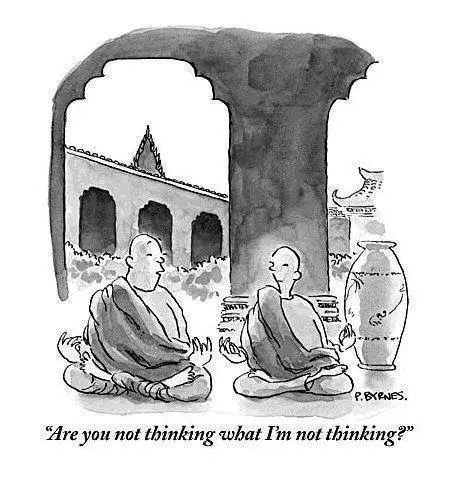
\includegraphics[width=7cm]{images/11_mindfulness.png}
\end{center}

\begin{leftindent}

A (\textit{sits in a perfect lotus seated position and looks to B in a requesting way})

B (\textit{sighs deeply and tries hard to somehow sit comfortably on the pillow without falling down or dislocating his hip})

A (\textit{closes the eyes with relish and takes a deep breath})

B (\textit{tries hard to keep up and takes a deep breath as well; which sounds more like a groan})

A (\textit{unctuous}): So? What do you feel?

B (\textit{opens the eyes; slightly in panic}): Feel? What should I feel?

A (\textit{gently}): Whatever is right now. What is right now?

B (\textit{confused}): What should be right now?

A (\textit{with godly patience}): What's in your body? What's in your thoughts? What kind of emotions are there?

B (\textit{completely overwhelmed}): Hmpf...

A (\textit{turns a gear down}): Can you feel your body?

B (\textit{clueless}): No.

A (\textit{still very patient}): ... your hands, the way they rest on your knees?

B (\textit{delighted}): Yes!

A (\textit{relieved}): Look, it's doable. And what's happening with your feelings?

B (\textit{suspiciously}): Which feelings?

A (\textit{pushy}): Well, the feelings you have right now.

B (\textit{categorically}): I don't have such a thing.
\end{leftindent}

\vspace{0.2cm}

Mindfulness is good and important, it lowers the blood pressure, makes a leader out of you, results in stable relationships, catapults you to enlightenment and much more. Everyone is practicing mindfulness these days!

To practice it, like we also do at Tantra retreats, is indeed required, because sometimes we don't know exactly what is meant with "being aware": Do I have to focus very strongly? On what exactly? How do I recognize that I am mindful right now?

Mindfulness training begins with something simple, something we always have with us in any case, and with which we are kind of familiar: our body: You can sit upright, maybe close your eyes, and feel whether you can sense something. For the beginning, that can be your breath or your heart beat. In case that works well already, you can be aware of warmth or coldness in different parts of your body, a tingling, a pull, tension, movement or pressure. With continuous practice more and more subtle sensations will emerge and you will be able to recognize reactions on impulses based on small body signals, like a small shivering, dizziness or a grumbling in your belly. This impulse can be something external, like the temperature or the words of someone else. It can also be something internal, like a thought or a feeling.

To turn one's attention to those impulses without judging them, clinging to them or turning into them is the key to many goodies, which mindfulness brings us over time. For example, a merry and unshakable serenity in daily life.
